
\documentclass[aps,prl,reprint]{revtex4-2}
\usepackage{gensymb}
\usepackage{graphicx}
\usepackage{amsmath}
\usepackage{hyperref}
\usepackage{dsfont}
\usepackage{relsize}
\usepackage{wrapfig}
\usepackage{graphicx}
\usepackage{hyperref}
\hypersetup{colorlinks=true, citecolor=blue, urlcolor=blue, linkcolor=blue}


\begin{document}

% Use the \preprint command to place your local institutional report
% number in the upper righthand corner of the title page in preprint mode.
% Multiple \preprint commands are allowed.
% Use the 'preprintnumbers' class option to override journal defaults
% to display numbers if necessary
%\preprint{}

%Title of paper
\title{Hall Effect Lab}

% repeat the \author .. \affiliation  etc. as needed
% \email, \thanks, \homepage, \altaffiliation all apply to the current
% author. Explanatory text should go in the []'s, actual e-mail
% address or url should go in the {}'s for \email and \homepage.
% Please use the appropriate macro foreach each type of information

% \affiliation command applies to all authors since the last
% \affiliation command. The \affiliation command should follow the
% other information
% \affiliation can be followed by \email, \homepage, \thanks as well.
\author{Trevor Smith, Alex Storrer}
\email[]{smith.tr@northeastern.edu}
\homepage[]{https://github.com/trevorm4x/}
%\thanks{}
%\altaffiliation{}
\affiliation{Northeastern University}


\date{\today}

\begin{abstract}
	Nothing is here
\end{abstract}


\maketitle

% body of paper here - Use proper section commands
% References should be done using the \cite, \ref, and \label commands
\section{Introduction}
% The Introduction should contain 1 or 2 paragraphs.
% Briefly state the physics underlying the experiment
% (what is being tested and why). 

\section{Apparatus}
% List equipment components (manufacturer, model
% numbers and brief specifications). 

The apparatus consisted of the following.
\begin{itemize}
\end{itemize}

\section{Efficiency of a Photovoltaic Cell}

\subsection{Procedure}
% Briefly describe the experimental procedures (in your own words, but don’t overdo it)
% Discuss calibrations, etc., if required
% Include necessary equations and put them on their own line (number them, e.g. “Eq. (3)”)
% Include plots showing relevant results (label each figure, e.g. “Fig. 3”, with caption).
% Describe what you found (describe what the plot illustrates)

\begin{figure}[h]
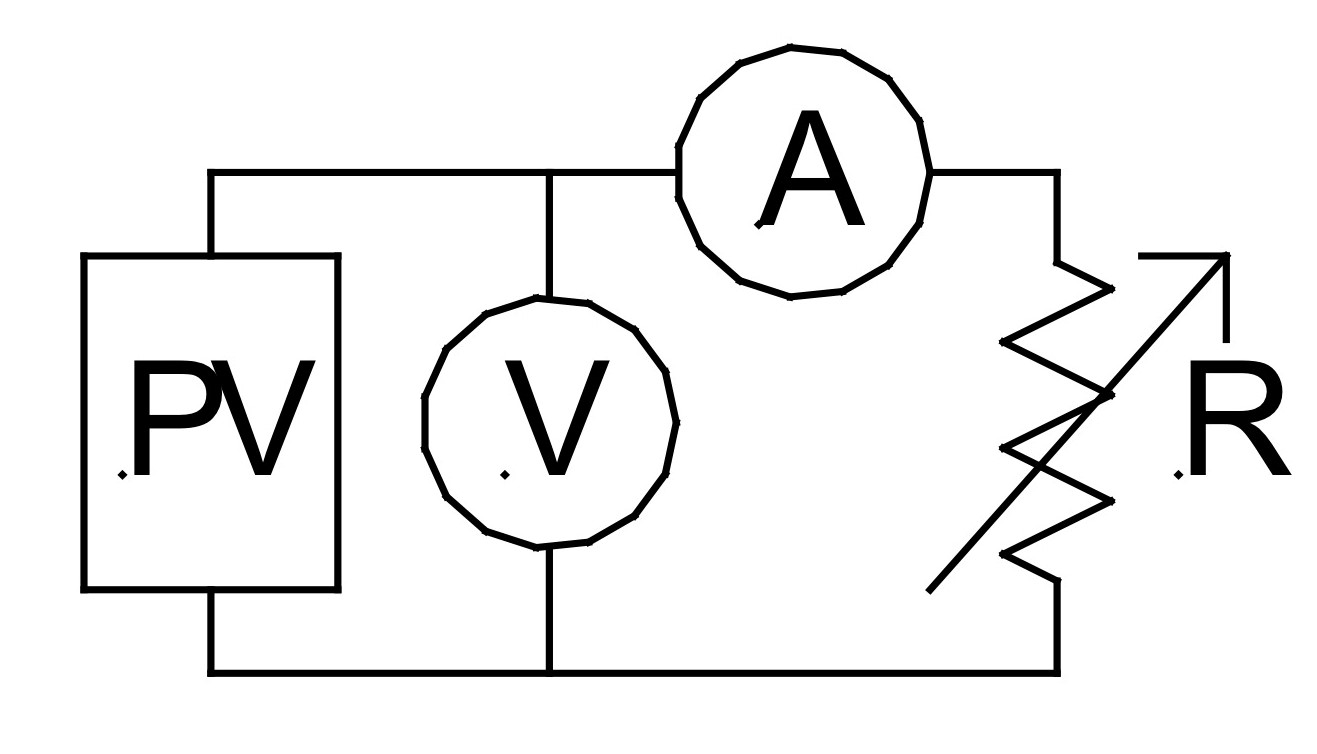
\includegraphics[width=0.4\textwidth]{../Images/l1_PartA.jpg}
\caption{\label{figA}Electrical circuit for measuring photovoltaic (PV) output voltage and current through a variable resistor (R). This curve reasonably matches theory.}
\end{figure}

\subsection{Results}

\newpage
\begin{equation}
    \mathlarger{\eta_{PV}}=P_E/P_L
    \label{eta_PV}
\end{equation}

\subsection{Conclusions}

\section{Summary}

\begin{widetext}
\begin{center}
\begin{table}[h]
\renewcommand{\arraystretch}{1.35}
\setlength{\tabcolsep}{10pt}
\caption{\label{}Measured and accepted values of the speed of light and refractive index of various materials.}
\begin{tabular}{|c|c|c|c|c|}
%\hline
\toprule
Apparatus &  $\eta$ (\%) & Accepted $\eta$ value & Refs. & Deviation \\
\colrule
Photovoltaic Cell &  $15 \pm 2$ & $17 \pm 2.5$ & \cite{Solar Cell} & $0\sigma$  \\
\colrule
Elecrolyzer &  $87 \pm 6$ & 80 & \cite{Electrolyzer} & $2\sigma$  \\
\colrule
Hydrogen Fuel Cell &  $49 \pm 5$ & 60 & \cite{Fuel Cell} & $-3\sigma$  \\
%\hline
\botrule
\end{tabular}
\end{table}
\end{center}
\end{widetext}





\begin{thebibliography}{9}
%
\bibitem{HHV} 
Wikipedia, Heat of Combustion: \\
\href{https://en.wikipedia.org/wiki/Heat_of_combustion}{https://www.wikepedia.com}
%
\bibitem{Solar Cell} 
Energysage, Most Efficient Solar Panels\\
\href{https://news.energysage.com/what-are-the-most-efficient-solar-panels-on-the-market/#:~:text=How%20efficient%20are%20solar%20panels,are%20not%20above%2020%25%20efficiency.}{https://www.energysage.com/}
%
\bibitem{Electrolyzer} 
Carbon Commentary, Hydrogen made by Electolysis\\
\href{https://www.carboncommentary.com/blog/2017/7/5/hydrogen-made-by-the-electrolysis-of-water-is-now-cost-competitive-and-gives-us-another-building-block-for-the-low-carbon-economy}{https://www.carboncommentary.com}
%

%
\bibitem{Fuel Cell} 
Energy.gov, Fuel Cell Fact Sheet\\
\href{https://www.energy.gov/sites/prod/files/2015/11/f27/fcto_fuel_cells_fact_sheet.pdf}{https://www.energy.gov}

\end{thebibliography}


\end{document}
%
% ****** End of file apstemplate.tex ******

